
%(BEGIN_QUESTION)
% Copyright 2006, Tony R. Kuphaldt, released under the Creative Commons Attribution License (v 1.0)
% This means you may do almost anything with this work of mine, so long as you give me proper credit

A tape-and-float system will be used to measure the level of an oil/water interface within a storage vessel:

$$\includegraphics[width=15.5cm]{i00517x01.eps}$$

The float itself needs to have the proper density to float on water yet sink in oil, so that it comes to rest (achieves neutral buoyancy) at the interface between the two liquids.  Your task is to make a float that will work for this application.

A hollow sheet-metal disk is the starting point for making the float.  It has a diameter of 21 inches and a height of 3 inches:

$$\includegraphics[width=15.5cm]{i00517x02.eps}$$

Although the float is hollow, there is a pipe plug on the top which may be removed, allowing you to insert lead pellets (``shot'') inside the float to make it heavier, thus changing its effective density.  Just by itself, without any lead shot, the float weighs 10 pounds.

Calculate how much lead shot to add to the float in order to achieve the right density so that it floats on the interface between the oil and the water.  Assume a specific gravity of 0.81 for the oil.

\vskip 10pt

Amount of lead shot to add inside the float = \underbar{\hskip 50pt} lbs

\vskip 10pt

Note: there is a {\it range} of correct answers to this problem.  You will receive full credit if your answer falls within this range.

\underbar{file i00517}
%(END_QUESTION)





%(BEGIN_ANSWER)

Amount of lead shot to add inside the float = \underbar{\bf 20.4 to 27.5} lbs

\vskip 10pt

10 points for correct answer, half-credit if the answer does not include the weight of the metal float (-10 pounds, for a range of 10.4 to 17.5 pounds shot weight)

%(END_ANSWER)





%(BEGIN_NOTES)

{\bf This question is intended for exams only and not worksheets!}.

%(END_NOTES)


